\documentclass[acmtog]{acmart}
\usepackage{graphicx}
\usepackage{subfigure}
\usepackage{natbib}

% Title portion
\title{Assignment 5 : Cloth Simulation with the Mass Spring System} 
\author{HONG YU \quad 2021533148 \quad hongyu@shanghaitech.edu.cn}

% Document starts
\begin{document}
\maketitle

\vspace*{2 ex}


\section{Introduction}

% Present background and related work of the algorithms required in this assignment. Summarize what you have done in this assignment.
% 在本次作业中我们完成了布料模拟的基本框架,包括质点系统的建立,质点系统的求解。在bonus部分,我们加入了风力的模拟,以及对布料和球体的碰撞检测。
In this assignment, we have implemented the basic framework for cloth simulation, including the establishment of a particle system and its solution. In the bonus section, we have incorporated wind force simulation and collision detection for both the cloth and spheres.

\section{Implementation Details}

% Consisely describe the working flow of algorithms. Elaborate on mathematical model and equations of each algorithm. Write down problems you met in the assignment and how you solve them.
\subsection{Mass Spring System}
% 首先我们建立了质点系统。我们在质点系统中定义了质点的性质,包含质量、速度、力、加速度。
% 对于弹簧,我们定义了性质stiffness,restlength以及dampingcoefficient。
% 在初始化particles的时候,我们赋值每个质点的质量,速度,力,加速度。在初始化弹簧的时候,我们链接了水平方向和竖直方向以及对角线方向的弹簧以及它们的方向。
First, we established the particle system. In the particle system, we defined the properties of particles, including mass, velocity, force, and acceleration.\\
For springs, we defined properties such as stiffness, rest length, and damping coefficient.\\
During the initialization of particles, we assigned values for the mass, velocity, force, and acceleration of each particle. When initializing springs, we connected springs in the horizontal, vertical, and diagonal directions, along with their respective orientations.

\subsection{Simulation}
% 在基础的模拟中,我们考虑了重力、空气阻力和弹簧的力。我们首先计算每个particle的受力。在计算弹簧力的部分,我们首先计算每个从particle发出的力,然后计算指向particle的力。
% 我们计算重力公式如下:
% 我们计算空气阻力的公式如下:
% 我们运用了胡克定律来计算弹簧的力。公式如下
In the basic simulation, we considered gravitational force, air resistance, and spring forces. We first calculated the forces acting on each particle. For the calculation of spring forces, we initially computed the forces originating from each particle and then determined the forces directed towards each particle.
\\
Formula for calculating gravitational force:
$$ G = mg$$

Formula for calculating air resistance:
$$ F_{air resistance} = -a*v$$

We applied Hooke's Law to calculate spring forces. The formula is as follows:
$$F_{hooke} = -k*(x_{current} - x_{rest}) $$

\subsection{Constraints}
% 为了给布料模拟增加限制,我们固定了左上角和右上角的particle。实现方法是每一次都跳过固定点的速度和position计算,最后将他们赋值为初始位置。
To impose constraints on the cloth simulation, we fixed the particles at the top-left and top-right corners. The implementation involved skipping the calculation of velocity and position for these fixed points at each iteration and, finally, assigning them their initial positions.

\subsection{Wind force}
% 在bonus中,我们增加了风力。我们把风力计算为一个恒定的vector。
In the bonus section, we introduced wind force. We calculated the wind force as a constant vector. The formula is as follows:
$$ F_{wind} = a * vector$$

\subsection{Sphere collision}
% 在bonus中,我们实现了布料和球的碰撞检测。
% 首先我们定义了一个虚拟的球,用中心和半径去定义一个空间中的虚拟的球。对于每个patricle,如果他和球心的距离小于等于半径,并且particle的速度和particle出发指向球心的向量的点乘为正,即particle的速度在指向球心的方向上有分量,我们认为即将发生碰撞。
% 我们通过更新速度来模拟碰撞。我们首先计算出particle和球心的距离,然后计算出particle的速度在指向球心的方向上的分量,然后将速度减去这个分量,即可模拟碰撞。
% 然后我们可视化了这个球。我们创建了sphere类,用来表示球。我们使用了经纬度的方法来创建球的顶点,然后连接这些vertex,用三角形来表示球的面。
% 然后我们调用了代码中给出的shader,来渲染球,具体渲染的方式可以参考我们第一次作业。
In the bonus section, we implemented collision detection between the cloth and a sphere.\\
Firstly, we defined a virtual sphere using its center and radius to represent a sphere in space. For each particle, if its distance to the sphere's center is less than or equal to the radius, and the dot product of the particle's velocity and the vector pointing from the particle to the sphere's center is positive (indicating that the particle has a component of velocity towards the sphere's center), we consider a collision is imminent.\\
We simulated the collision by updating the velocity. First, we calculated the distance between the particle and the sphere's center. Then, we computed the component of the particle's velocity in the direction of the vector pointing to the sphere's center. Subtracting this component from the velocity simulates the collision.\\
Additionally, we visualized the sphere by creating a Sphere class. We used latitude and longitude to generate the sphere's vertices and connected these vertices with triangles to represent the sphere's surface.\\
We then applied the provided shader in the code to render the sphere. The specific rendering approach can be referred to our first assignment.


\section{Results}

% Exhibit your results by figures and tables. You should give a brief description of each figure and table, e.g., how tables/figures prove the correctness of your algorithms.
% 我们展示了一些结果。我们首先展示了must部分的布料的模拟,然后展示了风力的模拟,最后展示了球体和布料的碰撞检测中的三个状态。
We presented some results, showcasing simulations of the cloth in the must-have part, wind force simulation, and three states during collision detection between the sphere and the cloth.

First, we demonstrated the simulation of the cloth in the must-have part.

Next, we showcased the simulation of wind force.
Finally, we displayed three states during collision detection between the sphere and the cloth.

\begin{figure}[H]
	\centering
	\subfigure[Must]{
		\label{Must}
		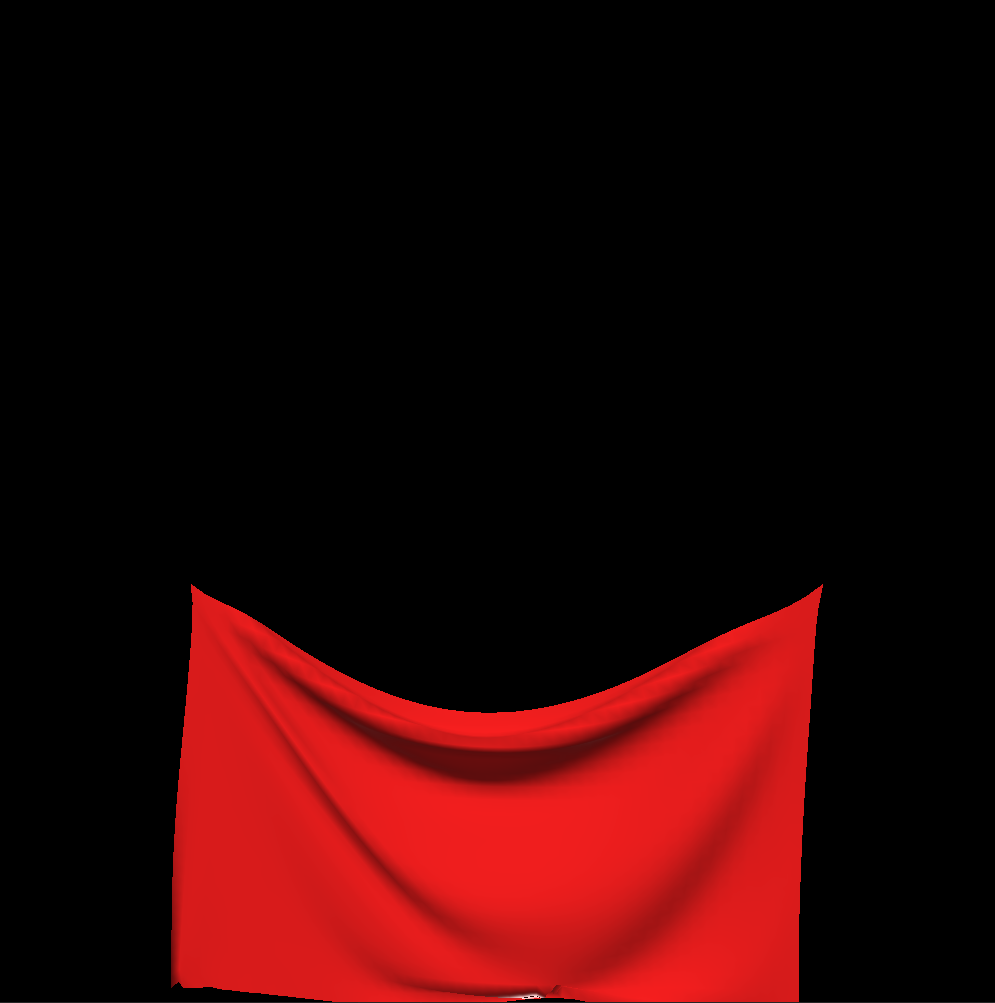
\includegraphics[width=0.2\textwidth]{must.png}}
	\subfigure[Wind Force]{
		\label{Porous Surface}
		
\includegraphics[width=0.2\textwidth]{wind.png}}
	\subfigure[Sphere Collision]{
		\label{Wine Glass}
		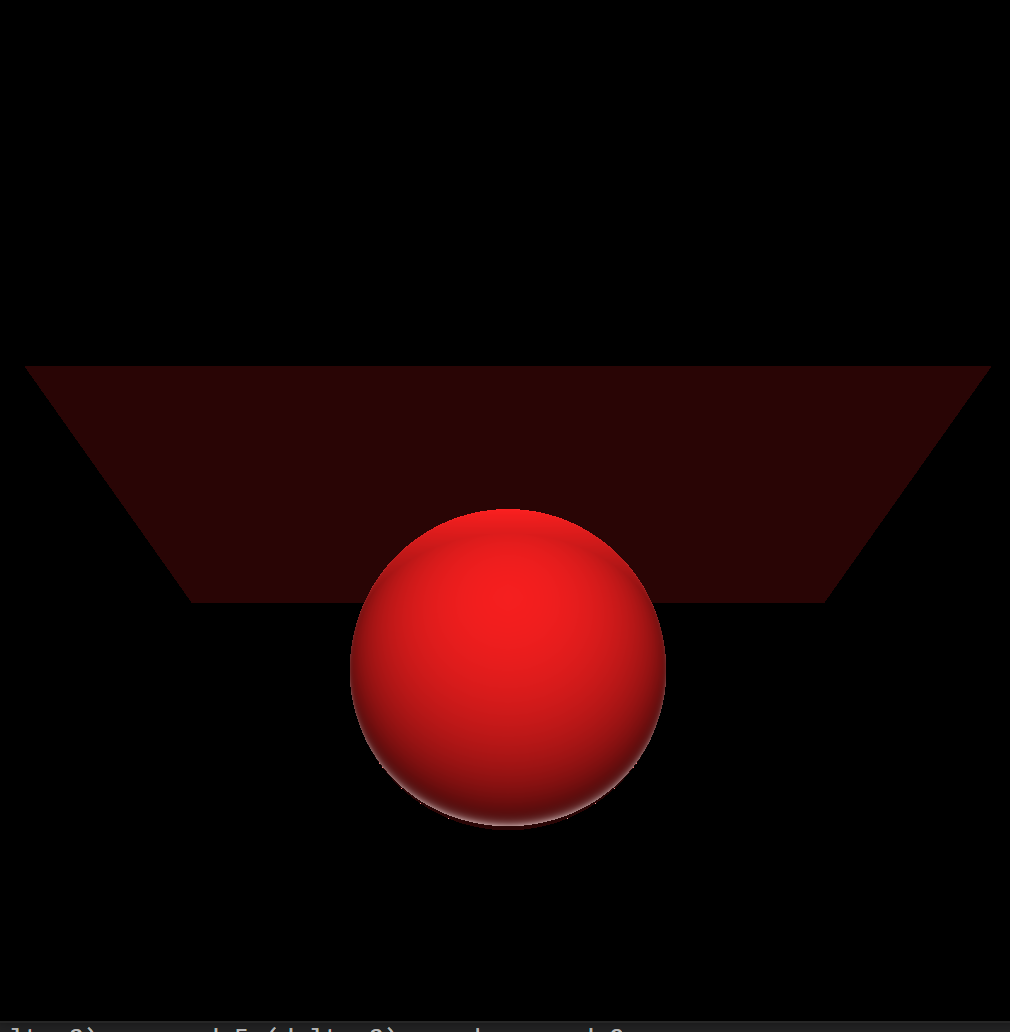
\includegraphics[width=0.2\textwidth]{sphere1.png}}
    \subfigure[Sphere Collision]{
        \label{Multi Surfaces}
        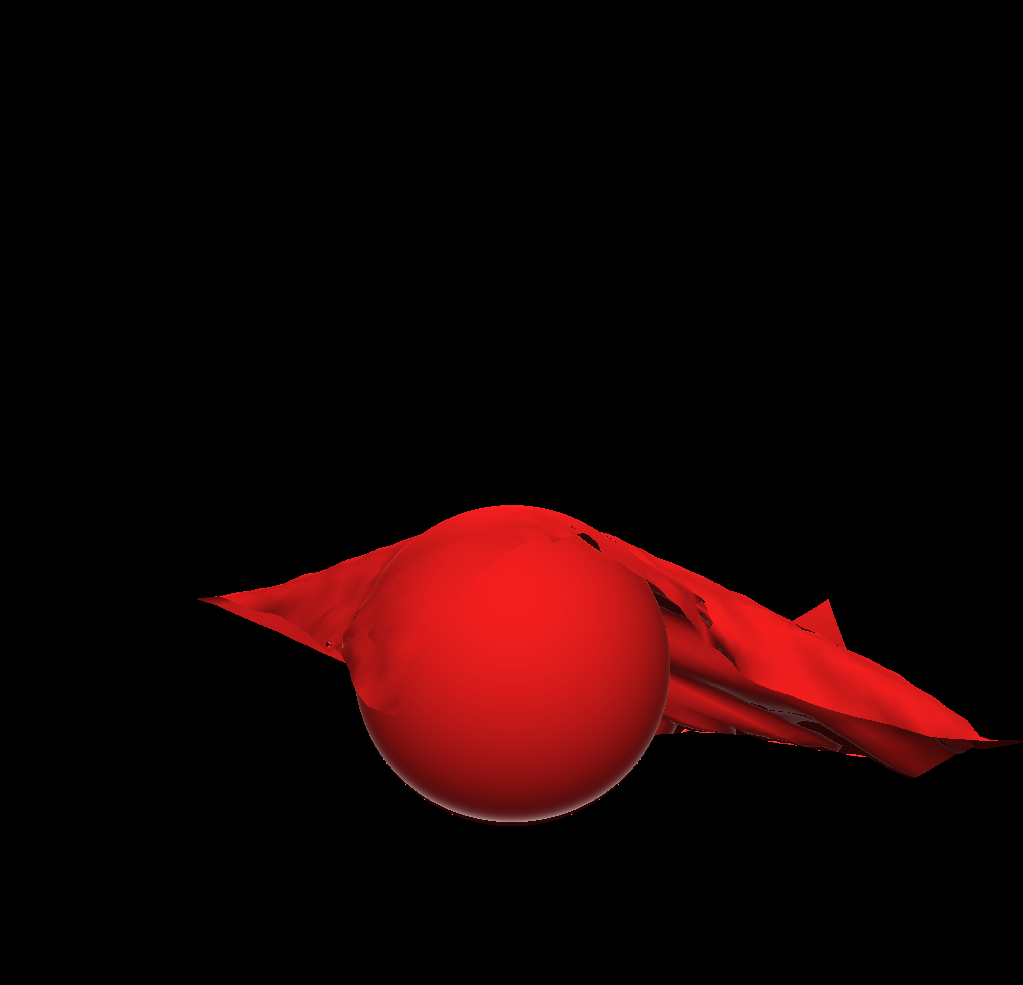
\includegraphics[width=0.2\textwidth]{sphere2.png}}
    \subfigure[Sphere Collision]{
        \label{Multi Surfaces}
        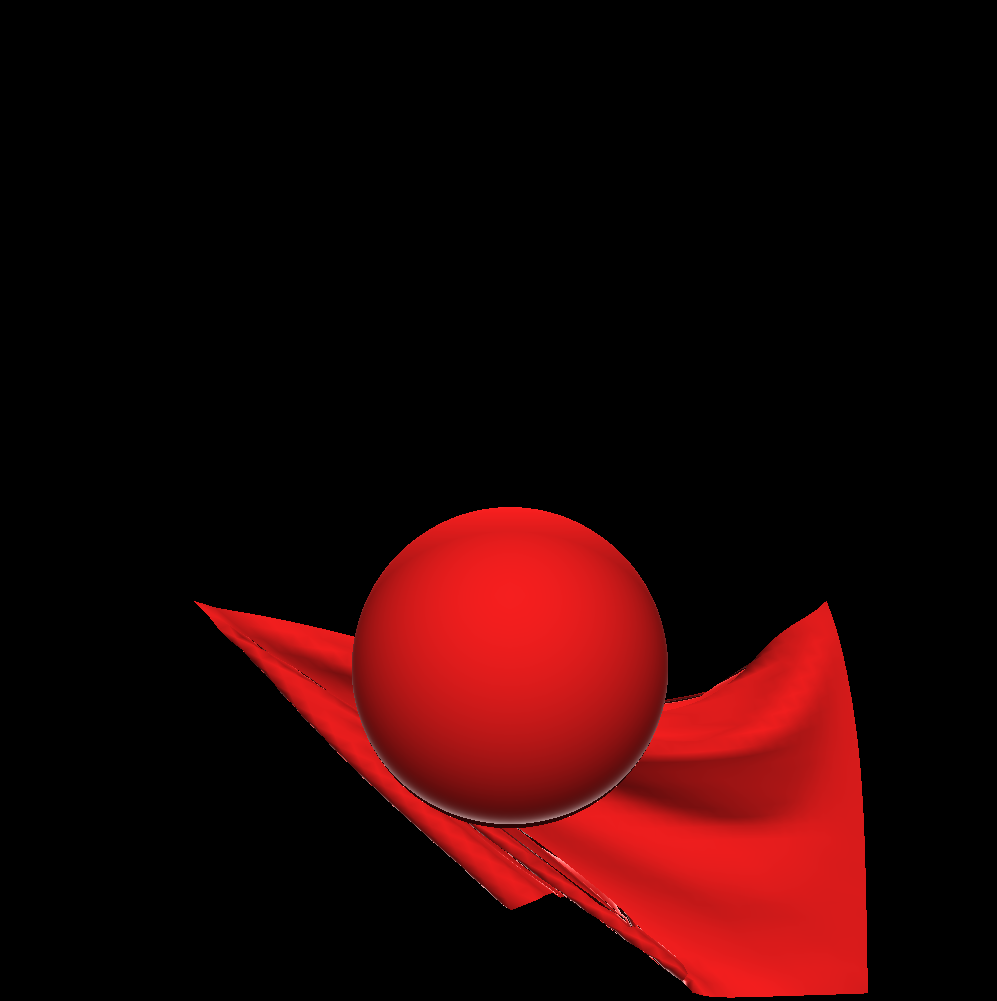
\includegraphics[width=0.2\textwidth]{sphere3.png}}
	\caption{Results}
	\label{Fig.main}
\end{figure}


\section{Conclusion}

% Draw a conclusion of this assignment.
% 在这次布料模拟中,我们把布料的模拟转化为对质点和弹簧系统的模拟。完成了must部分的布料模拟,以及bonus部分的风力模拟和球体和布料的碰撞检测。
In this cloth simulation, we transformed the simulation of the cloth into a simulation of a particle and spring system. We successfully implemented the must-have part of the cloth simulation, as well as the bonus sections involving wind force simulation and collision detection between a sphere and the cloth.

\end{document}
